\documentclass[11pt,a4 paper,one side]{article}
\usepackage{amsmath,amssymb,graphicx,subcaption}
\usepackage{ctex}  
\usepackage[colorlinks=true,linkcolor=red,citecolor=red,filecolor=magenta,urlcolor=cyan]{hyperref}
\usepackage{bookmark}
\usepackage{fontspec}
\setmainfont{Times New Roman}
\usepackage{xcolor}
\usepackage{geometry}
\geometry{a4paper, left=2.5cm, right=2.5cm, top=2.5cm, bottom=2.5cm}
\title{科学机器学习+HW1报告}
\author{2100012131 蒋鹏}
\date{\today}
\begin{document}
\maketitle
\tableofcontents
\section{问题描述}
对于计算区域$\Omega=[0,1]\times [0,1]$上的二维对流扩散方程\begin{equation}
    \frac{\partial c}{\partial t}+\nabla \cdot ([u;v]c) = \nabla \cdot(D\nabla c)
\end{equation}
其中$c(t,x,y)$代表物质浓度。速度场$[u;v]=[1;0]$,扩散系数$D=0.01$.初始条件满足$c(0,x,y)=0$。上下边界为周期边界条件,左边为入流条件满足\begin{equation}
    c(t,0,y)=\begin{cases}
        1,1/3<y<2/3 \\ 0,\text{其他}
    \end{cases}
\end{equation}
右边为出流条件,满足$\frac{\partial c(t,1,y)}{\partial \vec{n}}=0$,这里可以假设$c(t,x,y)=c(t,1,y)$当$x>1$.
\section{问题1}
采用有限体积方法,$dx=dy=0.005$,求解上述对流扩散方程,计算到$T=1.5$.
\subsection{计算格式}
这是一个关于空间导数为散度型的方程,进行有限体积推导,得到\begin{equation}
    c_{i,j}'\approx \frac{D}{h^2}(c_{i,j+1}+c_{i,j-1}+c_{i-1,j}+c_{i+1,j}-4c_{i,j})+\frac{c_{i-1/2,j}-c_{i+1/2,j}}{h}
\end{equation}
已知速度场分布,利用迎风格式近似中点函数值;再在时间方向上用一阶向前Euler离散,得到数值格式\begin{equation}
    c_{i,j}^{n+1} = \frac{Ddt}{h^2}(c_{i,j+1}^n+c_{i,j-1}^n+c_{i-1,j}^n+c_{i+1,j}^n-4c_{i,j}^n)+\frac{dt}{h}(c_{i-1,j}^n-c_{i,j}^n)
\end{equation}
\subsection{时间步长}
\paragraph{1}这是一个对流扩散方程,根据对流项的CFL条件和扩散方程的$L^2$稳定的Von Neumann条件:\begin{equation}
    \begin{cases}
        dt \leq dx \\ \frac{2Ddt}{h^2}\leq 1/2
    \end{cases}
\end{equation}
代入计算,得到$dt\leq 6.25e-4$,所以我们取$dt=5e-4$。
\paragraph{2} 若选择$dt=0.01$,在两个临界点$(0,1/3),(0,2/3)$的附近,解出现负数值,与物理背景实际不符;而在其他大范围内,解将会出现爆破,即数值上趋于$\infty$。
\subsection{结果展示}
以图片形式展示结果.\begin{figure}[htbp]
    \centering
    % 2x2 排列
    \begin{subfigure}{0.45\textwidth}
        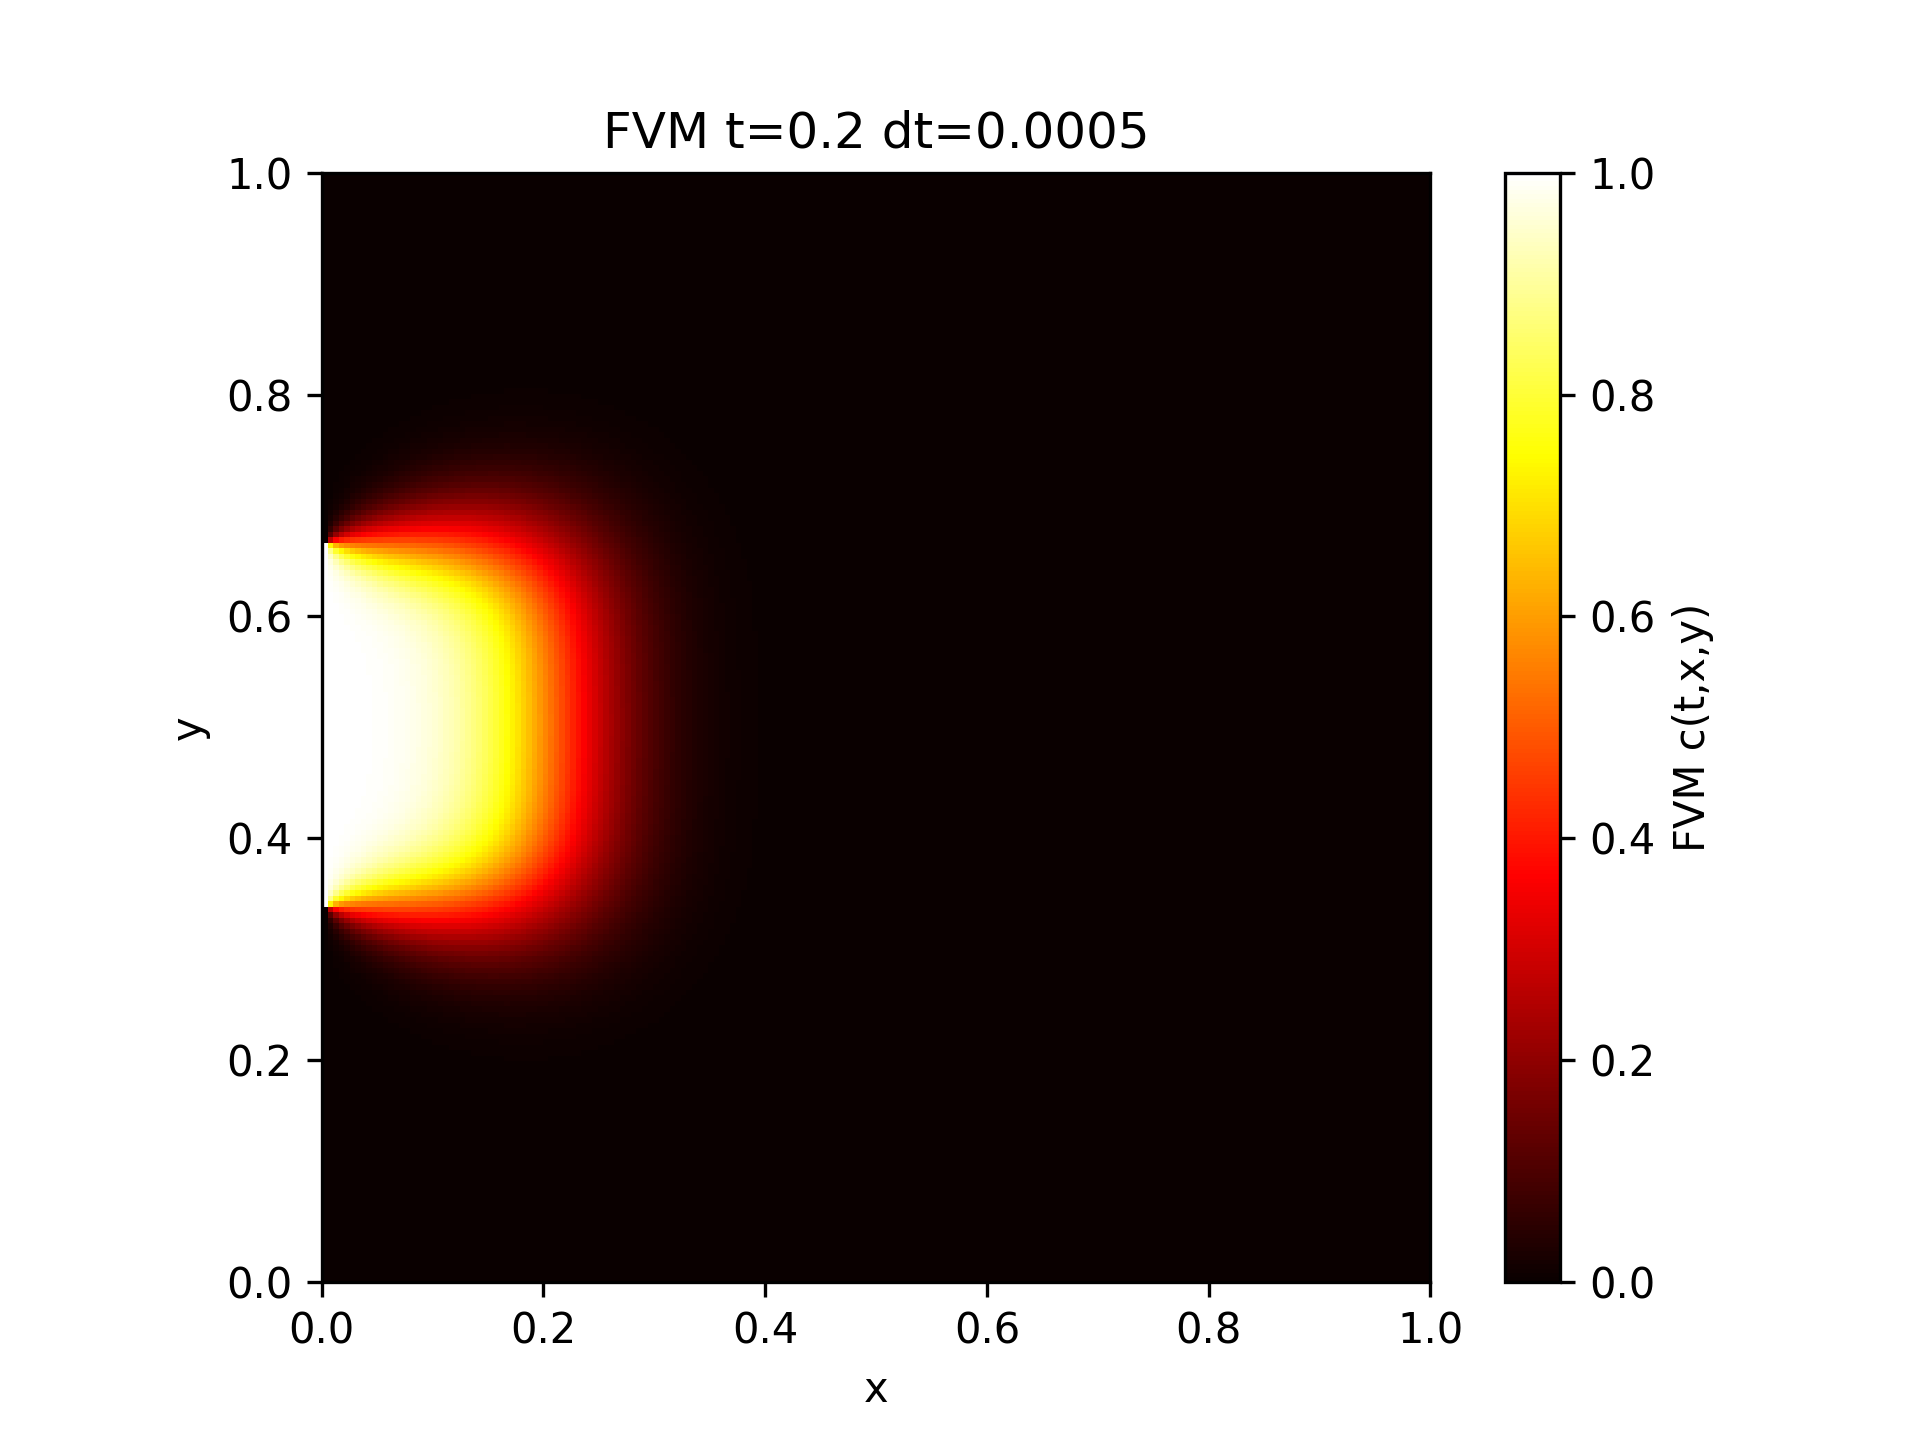
\includegraphics[width=\textwidth]{FVM t=0.2 dt=0.0005.png}
        \caption{FVM t=0.2 dt=0.0005}
        \label{FVM t=0.2 dt=0.0005}
    \end{subfigure}
    \hfill
    \begin{subfigure}{0.45\textwidth}
        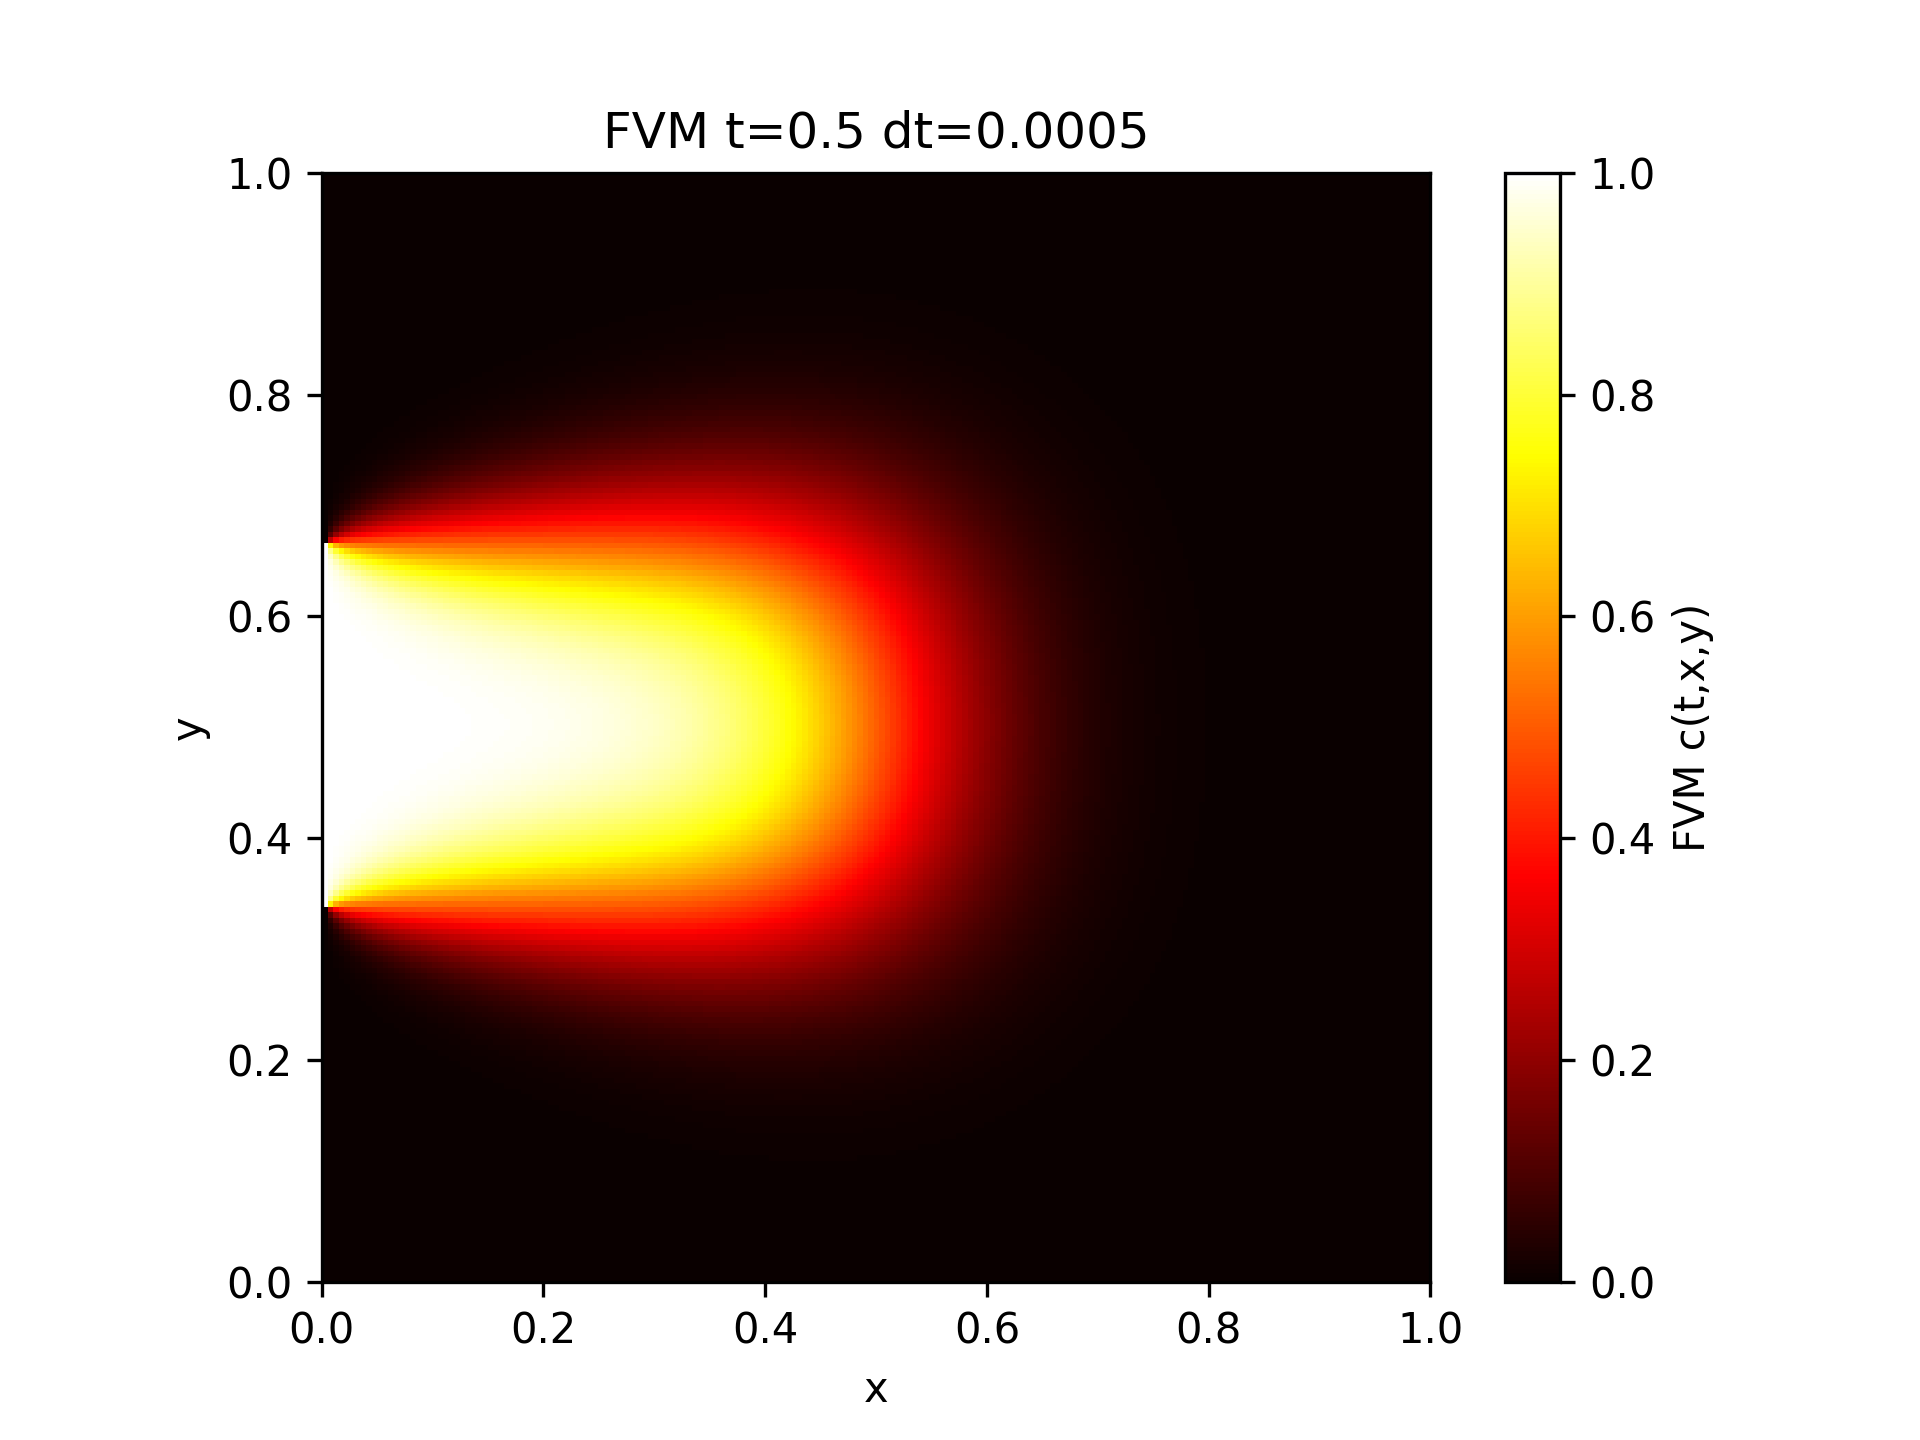
\includegraphics[width=\textwidth]{FVM t=0.5 dt=0.0005.png}
        \caption{FVM t=0.5 dt=0.0005}
        \label{FVM t=0.5 dt=0.0005}
    \end{subfigure}
    
    \vspace{0.5cm}  % 垂直间距
    
    \begin{subfigure}{0.45\textwidth}
        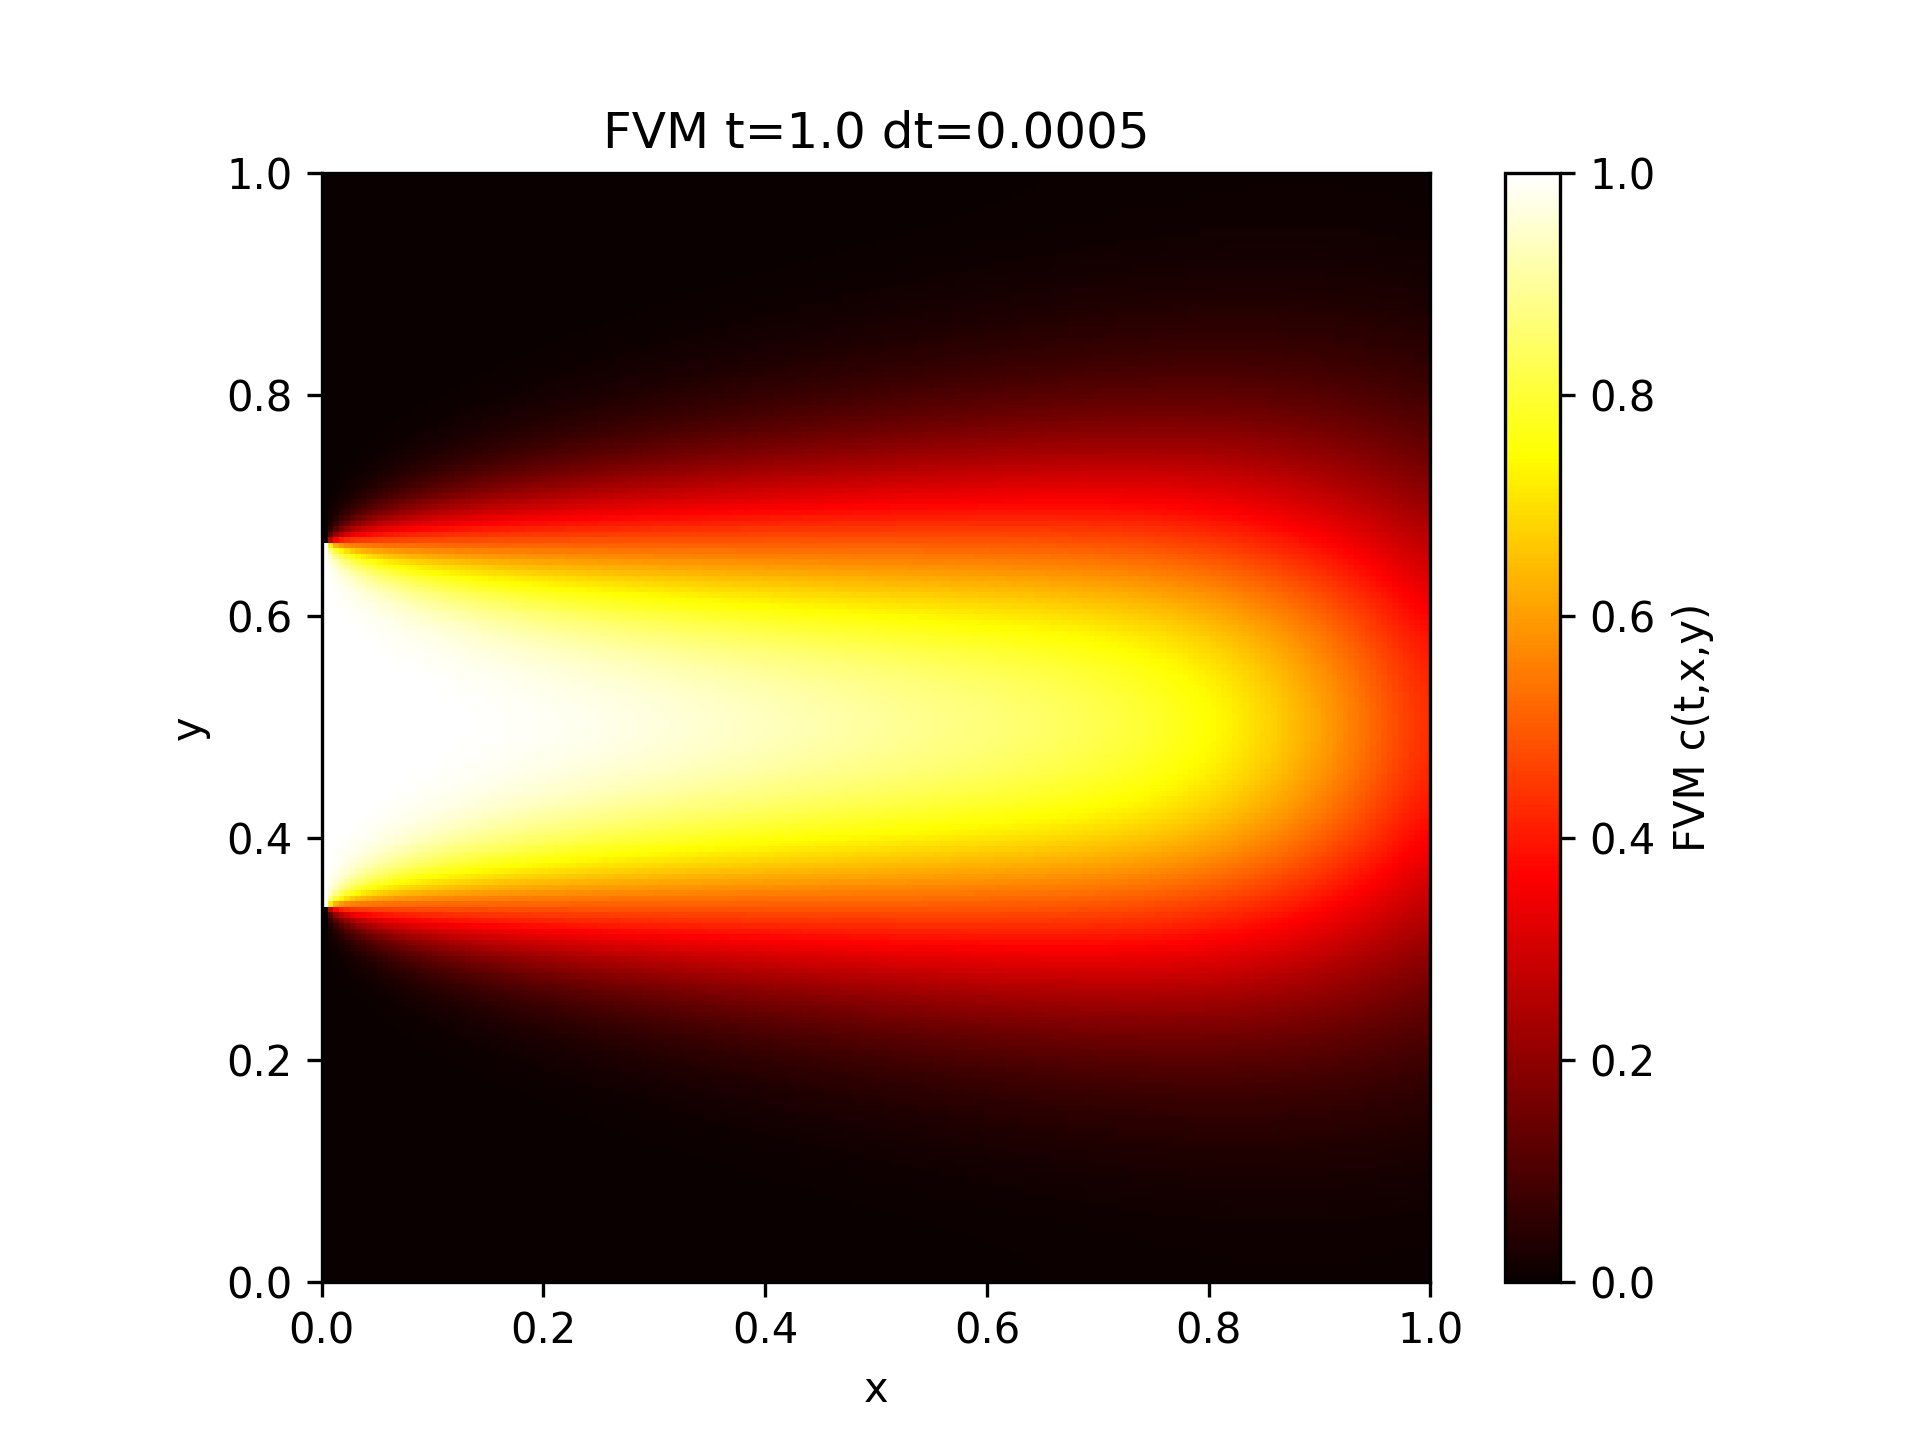
\includegraphics[width=\textwidth]{FVM t=1.0 dt=0.0005.png}
        \caption{FVM t=1.0 dt=0.0005}
        \label{FVM t=1.0 dt=0.0005}
    \end{subfigure}
    \hfill
    \begin{subfigure}{0.45\textwidth}
        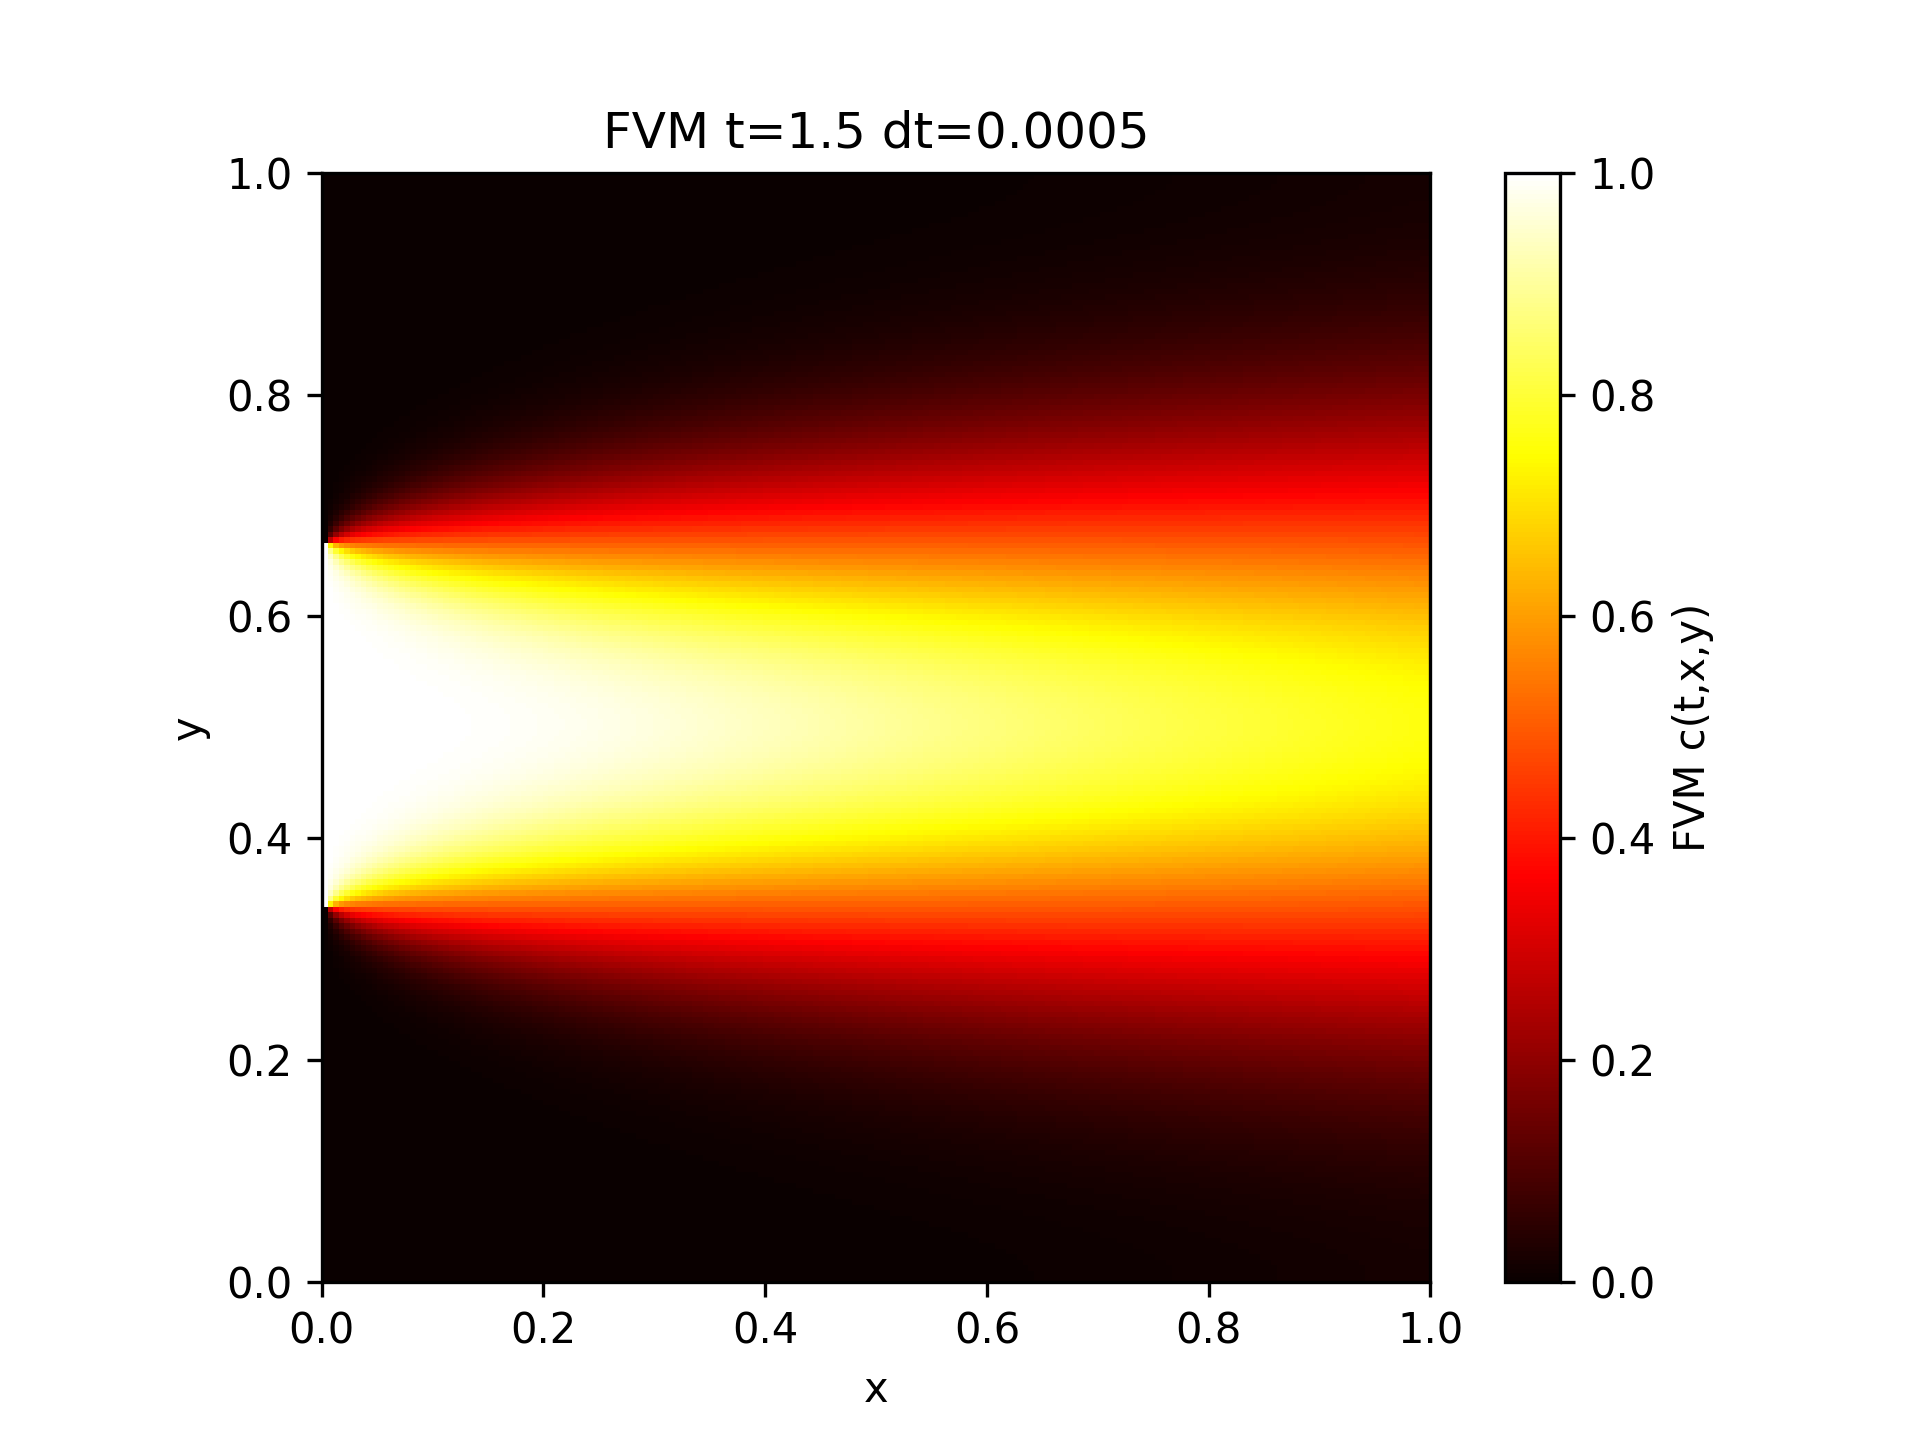
\includegraphics[width=\textwidth]{FVM t=1.5 dt=0.0005.png}
        \caption{FVM t=1.5 dt=0.0005}
        \label{FVM t=1.5 dt=0.0005}
    \end{subfigure}
    
    \caption{results of FVM}
    \label{results of FVM}
\end{figure}

\section{问题2}
采用基于正交分解的降阶模型对上述问题进行计算.首先写出离散后的方程\begin{equation}
    \frac{\partial \vec{c}}{\partial t} = A\vec{c}+f
\end{equation}
其中$A$是对流扩散方程离散后的矩阵,$f$是边界条件的作用。
\section{问题3}
\end{document}